\documentclass[12pt]{article}
\usepackage{geometry}
\geometry{a4paper}
\usepackage[colorlinks, linkcolor=blue, citecolor=blue, urlcolor=blue]{hyperref}
\usepackage[automake]{glossaries-extra}
\usepackage{appendix}
\usepackage{graphicx} % Needed for including images
\usepackage{mdframed} % For creating framed boxes
\usepackage[backend=biber, style=ieee]{biblatex} % Adding biblatex with IEEE style
\usepackage{minted}

\addbibresource{Reference.bib} % Specify the bibliography file, here 'references.bib'


\makeglossaries % 初始化术语表系统

% 定义一些术语
 
\newglossaryentry{opencv}{
    name=OpenCV,
    description={OpenCV (Open Source Computer Vision Library) is a library of programming functions mainly for real-time computer vision. Originally developed by Intel, it was later supported by Willow Garage, then Itseez (which was later acquired by Intel). The library is cross-platform and licensed as free and open-source software under Apache License 2. Starting in 2011, OpenCV features GPU acceleration for real-time operations.\cite{qt}}
}

\newglossaryentry{QT}{
    name=Qt,
    description={Qt (pronounced "cute" or as an initialism) is cross-platform application development framework for creating graphical user interfaces as well as cross-platform applications that run on various software and hardware platforms such as Linux, Windows, macOS, Android or embedded systems with little or no change in the underlying codebase while still being a native application with native capabilities and speed.\cite{cv}}
}

\newglossaryentry{aruco}{
    name=Aruco Marker,
    description={ArUco markers are 2D binary-encoded fiducial patterns designed to be quickly located by computer vision systems. ArUco marker patterns are defined by a binary dictionary in OpenCV, and the various library functions return pattern IDs and pose information from scanned images.\cite{arucomarkers}}
}

\newglossaryentry{vtk}{
      name=VTK,
      description={The Visualization Toolkit (VTK) is an open-source, freely available software system for 3D computer graphics, modeling, image processing, volume rendering, scientific visualization, and 2D plotting. It supports a wide variety of visualization algorithms and advanced modeling techniques, and it takes advantage of both threaded and distributed memory parallel processing for speed and scalability, respectively.\cite{vtkBook}}
}

\newglossaryentry{alpha}{
      name=Alpha Blending,
      description={In computer graphics, alpha compositing or alpha blending is the process of combining one image with a background to create the appearance of partial or full transparency. It is often useful to render picture elements (pixels) in separate passes or layers and then combine the resulting 2D images into a single, final image called the composite. Compositing is used extensively in film when combining computer-rendered image elements with live footage. Alpha blending is also used in 2D computer graphics to put rasterized foreground elements over a background.\cite{Alpha}}
}

\newglossaryentry{aesl}{
      name=Adaptive Exponential Smoothing,
      description={Adaptive exponential smoothing models are designed to improve performance by letting the smoothing parameter vary according to the most recent forecasting accuracy. \cite{aes,aes2}}
}

\newglossaryentry{emal}{
      name=Exponential Moving Average,
      description={An exponential moving average (EMA) is a type of moving average (MA) that places a greater weight and significance on the most recent data points. The exponential moving average is also referred to as the exponentially weighted moving average. An exponentially weighted moving average reacts more significantly to recent price changes than a simple moving average simple moving average (SMA), which applies an equal weight to all observations in the period.\cite{InvestopediaEMA}}
}

\newglossaryentry{cesl}{
      name=Complex Exponential Smoothing,
      description={Complex exponential smoothing is a time series forecasting method that combines exponential smoothing with trend and seasonality. It is a variant of the standard exponential smoothing method, which is a simple technique for smoothing out data by using a weighted average of past observations.\cite{ComplexES2018}}
}


\newglossaryentry{mrtkl}{
      name=Microsoft Mixed Reality Toolkit-Unityde,
      description={MRTK-Unity is a Microsoft-driven project that provides a set of components and features, used to accelerate cross-platform MR app development in Unity. Here are some of its functions: 1.Provides the cross-platform input system and building blocks for spatial interactions and UI. 2.Enables rapid prototyping via in-editor simulation that allows you to see changes immediately. 3.Operates as an extensible framework that provides developers the ability to swap out core components.\cite{MRTKUnity2024}}
}

\newglossaryentry{blender}{
      name=Blender,
      description={Blender is a free and open-source 3D computer graphics software tool set used for creating animated films, visual effects, art, 3D-printed models, motion graphics, interactive 3D applications, virtual reality, and, formerly, video games. Blender's features include 3D modelling, UV mapping, texturing, digital drawing, raster graphics editing, rigging and skinning, fluid and smoke simulation, particle simulation, soft body simulation, sculpting, animation, match moving, rendering, motion graphics, video editing, and compositing\cite{Blender2024,blender}.}
}

\newglossaryentry{holo}{
      name=Microsoft Hololens,
      description={Microsoft HoloLens is an augmented reality (AR)/mixed reality (MR) headset developed and manufactured by Microsoft. HoloLens runs the Windows Mixed Reality platform under the Windows 10 operating system. Some of the positional tracking technology used in HoloLens can trace its lineage to the Microsoft Kinect, an accessory for Microsoft's Xbox 360 and Xbox One game consoles that was introduced in 2010\cite{holo1,holo2}}
}

\newglossaryentry{git}{
      name=GitHub,
      description={GitHub is a developer platform that allows developers to create, store, manage and share their code. It uses Git software, providing the distributed version control of Git plus access control, bug tracking, software feature requests, task management, continuous integration, and wikis for every project. Headquartered in California, it has been a subsidiary of Microsoft since 2018. It is commonly used to host open source software development projects. As of January 2023, GitHub reported having over 100 million developers and more than 420 million repositories, including at least 28 million public repositories. It is the world's largest source code host as of June 2023.\cite{git}}
}

% 定义一个缩写词
\newabbreviation{aes}{AES}{
      Adaptive Exponential Smoothing}

\newabbreviation{ema}{EMA}{
      Exponential Moving Average}

\newabbreviation{ces}{CES}{
      Complex Exponential Smoothing}    

\newabbreviation{mrtk}{MRTK}{
      Microsoft Mixed Reality Toolkit-Unity}    
      

\begin{document}

\begin{titlepage}
      \centering

      \includegraphics[width=0.6\textwidth]{Liverpool.jpg} % Increased width
      \vspace*{1cm}

      \Large
      COMP390

      \large
      2023/24

      \vspace{0.5cm}
      \Huge
      \textbf{Computer Vision and AR for Endovascular Intervention}

      \vspace{1.5cm}


      % Framed box for student information
      \begin{mdframed}
            \normalsize % Smaller text size within the box
            \textbf{Student Name:} [Yulin Huang]\\[20pt] % Name on the same line, add vertical space
            \textbf{Student ID:} [201676465]\\[20pt] % ID on the same line, add vertical space
            \textbf{Supervisor Name:} [Anh Nguyen] % Supervisor on the same line
      \end{mdframed}

      \vspace{2cm} % Adjust space as necessary
      \Large
      \textbf{DEPARTMENT OF}\\
      \vspace{0.1cm} % Adjust line spacing
      \textbf{COMPUTER SCIENCE}

      \vspace{4cm} % Large space as required
      \large
      University of Liverpool\\
      Liverpool L69 3BX


\end{titlepage}
% Acknowledgements page
\newpage
\thispagestyle{empty} % Remove page number from the acknowledgements page
\begin{center}
      \Large \textbf{Acknowledgements}
\end{center}
\vspace{1cm}
\normalsize
%Here for the Acknowledgements
I would like to express my deepest gratitude to my supervisor, Anh Nguyen, for his invaluable guidance and support throughout my research. His insights and expertise have been fundamental to the success of this work.
\\\\
Special thanks also go to Tudor Jianu for his advice and contributions that greatly enhanced this project.
\\\\
I would like to extend my heartfelt thanks to my family. Their unwavering support and love have been my strength and motivation throughout this journey.
\\\\
I am also immensely grateful to my girlfriend, Lucy Zhao, for her understanding and encouragement during the course of my thesis. Her support has been a cornerstone of my personal and academic journey.
\\\\
Furthermore, I wish to acknowledge the critical role played by open-source libraries in the realization of this project. I extend my thanks to the developers of OpenCV\cite{opencv_library} and SciKit-Surgery Augmented Reality\cite{Thompson_SciKit-Surgery_Compact_Libraries_2020} for providing essential tools and references that significantly contributed to my project.
\\\\
This work would not have been possible without the collective support and encouragement from each of these individuals and resources. Thank you.
\newpage
\begin{titlepage}
      \centering


      \includegraphics[width=0.6\textwidth]{Liverpool.jpg} % Increased width
      \vspace*{1cm}

      \Large
      COMP390
      \large
      2023/24

      \vspace{4.5cm}
      \Huge
      \textbf{Computer Vision and AR for Endovascular Intervention}

      \vspace{1.5cm}



      \vspace{4cm} % Adjust space as necessary
      \Large
      \textbf{DEPARTMENT OF}\\
      \vspace{0.1cm} % Adjust line spacing
      \textbf{COMPUTER SCIENCE}

      \vspace{1cm} % Large space as required
      \large
      University of Liverpool\\
      Liverpool L69 3BX

\end{titlepage}
\tableofcontents
\newpage

% Abstract 
\section*{Abstract}
This section should contain a concise summary of the document content.
% Statement of Ethical Compliance
\section*{Statement of Ethical Compliance}
\begin{mdframed}
      \Large % Larger font size for the first two lines
      Data Category: A \\
      Participant Category: 0 \\
      \normalsize % Normal font size for the rest of the text
      I confirm that I have read the ethical guidelines and will follow them during this project. Further details can be found in the relevant sections of this proposal.
\end{mdframed}
\newpage

% Introduction & Background
\section{Introduction \& Background}



\section{Design \& Implementation}

\subsection{Part1: Real-world Model Interaction and Tracking}
% 这一部分集中讨论与现实世界模型的交互与跟踪的设计和实现。

In this part, I used \gls{opencv}\cite{opencv_library} and SciKit-Surgery Augmented Reality\cite{Thompson_SciKit-Surgery_Compact_Libraries_2020} libraries for image
processing and  model tracking. \gls{QT}\cite{QtWebsite} is used to design the graphical interface, and also \gls{vtk}\cite{vtkBook}. OpenCV and SciKit-Surgery libraries help me process images
and track \gls{aruco}\cite{1467495} within video steaming. Qt allows me to create a user interface that ensures  user could more easily change multiple settings, which can enhance the user experience.
VTK and SciKit-Surgery Augmented Reality library are the management of overlay and multi-layer video rendering in my project.
An ArUco Marker Generator is also included, which enables the user to generate different ArUco Markers and save them.
This section will detail the system's design, focusing on System Components and Organization, Data Structures and Algorithms,
User Interface Design, and Design Notation and Diagrams.


\subsubsection{Design}
\begin{enumerate}
      \item \textbf{System Components and Organization}
            \\The project is structured into three primary components, each responsible for distinct functionalities within the system.
            Here’s a detailed breakdown of these components and their organization:
            \begin{enumerate}
                  \item \textbf{Frontend - User Interface}
                        \\The system's user interface is developed using Qt, which is a framework that enables the creation of graphically applications.
                        The main class controlling the UI is \emph{Overlay\_and\_Tracking.py}, which serves as the central hub for user interactions and display functionalities.
                        This class manages the overlay of models on video streaming and provides interactive buttons for users to control various settings, such as model color,
                        video source, models uploading and changing, or adjusting ArUco marker types and sizes, and more.
                  \item \textbf{Backend - Helper Classes}
                        \\The backend is composed of various helper classes, each set to handle specific tasks:
                        \begin{itemize}
                              \item \textit{Image Capture:} The \emph{video\_source.py} class handles the acquisition of video streams from various sources,
                                    including live cameras and recorded media. It is responsible for configuring camera settings, initializing video capture, and video frame cropping to adapted to screen size. This component ensures the reliability and stability of video feed intake.

                              \item \textit{Model Loading:} Managed by \emph{model\_loader.py}, this component is important for the model loading and initializing. It loads ".stl" model files from external files, sets up texture mapping, and prepares the models for real-time overlay. The class also checks for errors in model data to prevent crashes or rendering issues during operation. It also optimizes the structures of model data to enhance rendering efficiency and reduce memory overhead.

                              \item \textit{Model Overlay:} The \emph{overlay\_window.py} is central to integrating 3D models with live or recorded video. With the help of VTK, this module could set up a multi-layered rendering environment where each layer can independently handle elements like video backgrounds, 3D models, or some GUI overlays(In the future, maybe.).

                              \item \textit{Transform Management:} The \emph{transform\_manager.py} class provides a method for managing 4x4 transformation matrices crucial for spatial adjustments of models in 3D space. It stores and retrieves transformations efficiently. And allow it for dynamic modifications of object orientations and positions.

                              \item \textit{ArUco Marker Tracking:} Functionality provided by \emph{arucotracker.py} includes detecting and decoding ArUco markers from the video stream using OpenCV. This module calculates position and orientation of detected marker, and handle the spatial position data for model tracking.
                        \end{itemize}


                  \item \textbf{Additional Component - ArUco Marker Generator}
                        \\An independent component in the system is the ArUco Marker Generator, managed by \emph{Aruco\_Generator.py}.
                        This tool allows users to select and visualize different ArUco markers. Users can also save these markers as separate image files.
            \end{enumerate}
            \paragraph{Organization:\\}
            The system’s architecture is designed to easy maintenance and scalability.
            The modular nature of the helper classes allows for isolated development and testing,
            which enhances the system's robustness and flexibility.
            This organization simplifies development and testing
            and enables the integration of additional functionalities in the future with minimal disruption to the existing system.



      \item \textbf{User Interface Design}
            \\
            In this section, I will show the user interface design of the two main applications of my Part1. Both applications use the Python-based Qt package for user GUI design.
            I will also provide a brief description of the Main menu and the ArUco Marker Generator interface.
            Screenshots of the main layout and main interface will be included in the (a) Main Menu (Overlay and Tracking) and (b) ArUco Generator sections, and screenshots of settings and functionality will be listed separately in the (c) Screen Mockups, Sketches, and Screenshots section.
            \begin{enumerate}
                  \item \textbf{Main Menu(Overlay and Tracking)}
                        % 描述主菜单的设计和功能。
                        \begin{figure}[H]
                              \centering
                              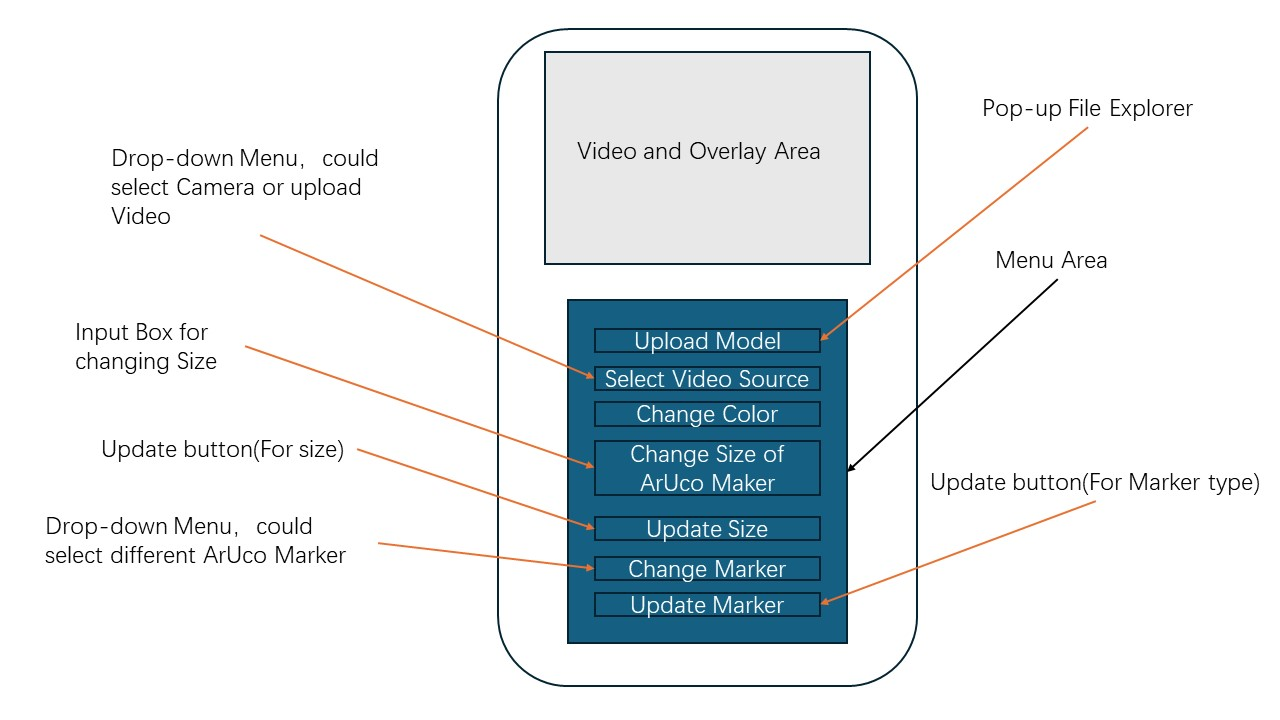
\includegraphics[width=1.2\textwidth]{design_overlay.jpg}
                              \caption{Design of Overlay and Tracking Main Menu}
                        \end{figure}

                        \begin{figure}[H]
                              \centering
                              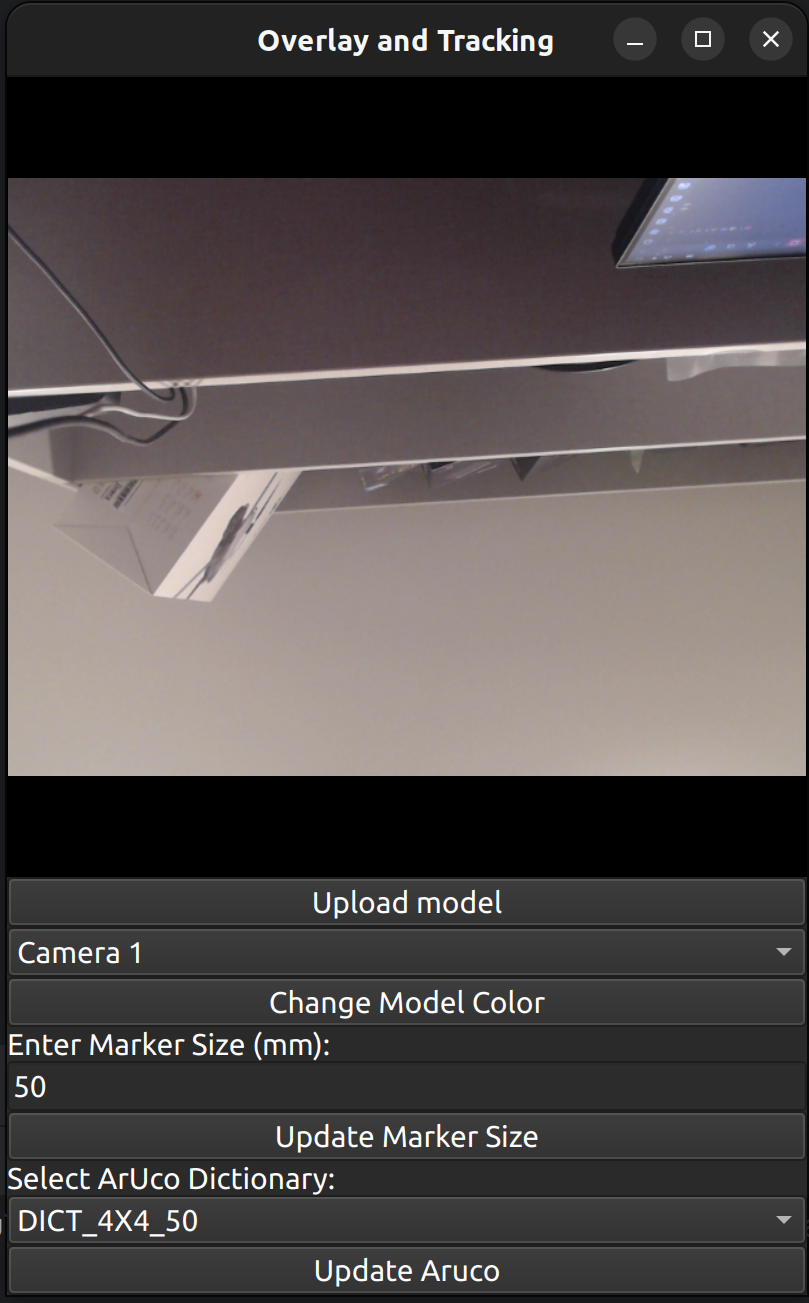
\includegraphics[width=0.4\textwidth]{main_page.png}
                              \caption{Overlay and Tracking Main Menu(Without Overlay Activated)}
                        \end{figure}
                        The main menu of Overlay and Tracking is the central hub of the application, providing users with access to all the functionalities.
                        The Main Menu consists of the Video and Overlay Area, which displays the video image and overlay of the model, and the Menu Area, which is responsible for setting various parameters.
                        The menu includes buttons for model uploading, video source selection, ArUco marker settings, and model color adjustments.
                        \\\\
                        When you click on the "Upload Model" button, a file explorer will pop up to select the folder where you want to upload the model. The program will read two files in the folder, one is the model file in ".stl" format, and the other is a file named "colours.txt". the first field in the txt file is the file name of the model, and the last three fields are The first field in the txt file is the file name of the model, and the last three fields are the RGB data of the default colours of the model (the model colours can be changed in the application interface after uploading). After uploading the model will be overlayed onto the video display as Overlay. The second button is the video source selection button, when clicked, a drop-down menu with three options will appear, "Camera1", "Camera2" and "Upload Video Camera1", "Camera2" and "Upload Video". The app will default to "Camera1" as the video source when it is initially launched. Selecting "Camera1" or "Camera2" will directly switch to the corresponding video source. After selecting the "Upload Video" option, an "Upload Video File" button will appear at the bottom. Clicking on the "Upload Video File" button will start the file explorer, you can select ".mp4", ".avi", ".webm" format video for uploading. After the video has been uploaded the tracking of Overlay and ArUco markers will start automatically if there is already an uploaded model present. Similarly, the video source can be switched back to the Camera input by selecting Camera1. After uploading the model, you can change the colour of the model by clicking the "Change Model Color" button.
                        \\\\
                        To ensure the accuracy of ArUco marker tracking, you need to modify the "ArUco Dictionary" to the corresponding dictionary of the marker you are using and click "Update ArUco "button. You also need to change the "ArUco Marker Size", which represents the size of the real ArUco marker in millimetres, and click the "Update Marker Size" button when you are done.

                  \item \textbf{ArUco Generator}
                        % ArUco生成器设计图
                        \begin{figure}[H]
                              \centering
                              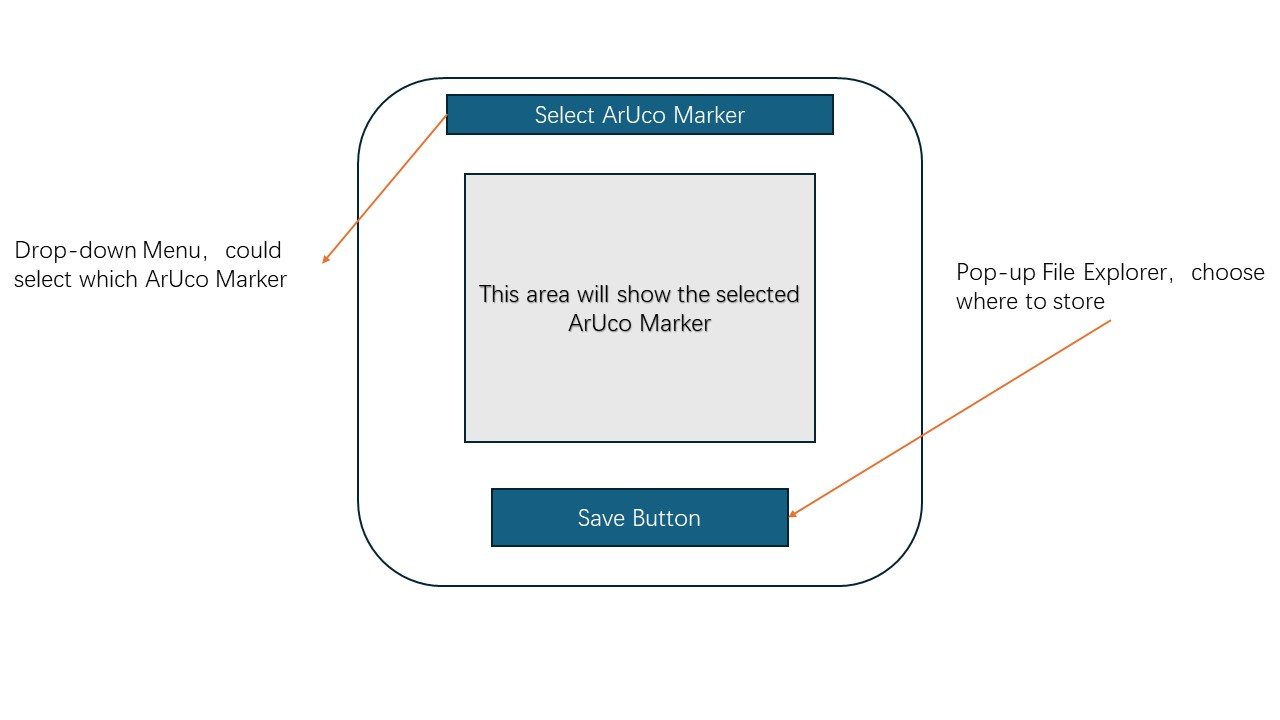
\includegraphics[width=1.2\textwidth]{design_generator.jpg}
                              \caption{Design of ArUco Generator}
                        \end{figure}
                        % 描述ArUco生成器的设计和功能。
                        \begin{figure}[H]
                              \centering
                              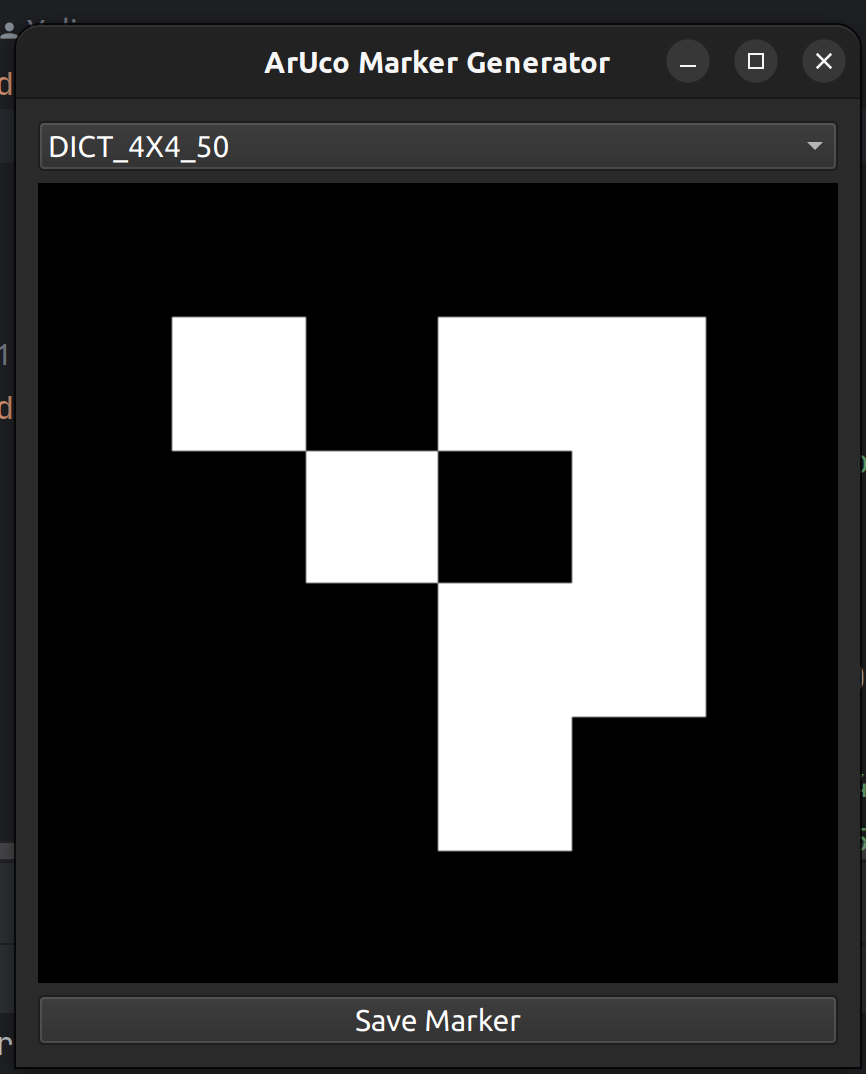
\includegraphics[width=0.4\textwidth]{main_arucuo.png}
                              \caption{ArUco Generator}
                        \end{figure}
                        The ArUco Generator interface allows users to select different ArUco markers from a predefined list and visualize them in real-time.
                        The interface provides a clear preview of the selected marker and allows users to save the marker as an image file for later use.
                        The design is simple and user-friendly, with intuitive controls for easy marker customization.
                        \\\\
                        You can first select the ArUco marker you want to use by launching the drop-down menu via "Select Aruco" and the selected ArUco marker will be displayed on the screen in real time. After that, you can click the "Save Marker" button to start the file explorer to save the marker, the file name will be set to the corresponding dictionary of the ArUco marker by default.

                  \item \textbf{Screenshots of Settings and Functionality}
                        % Overlay截图展示
                        \begin{figure}[H]
                              \centering
                              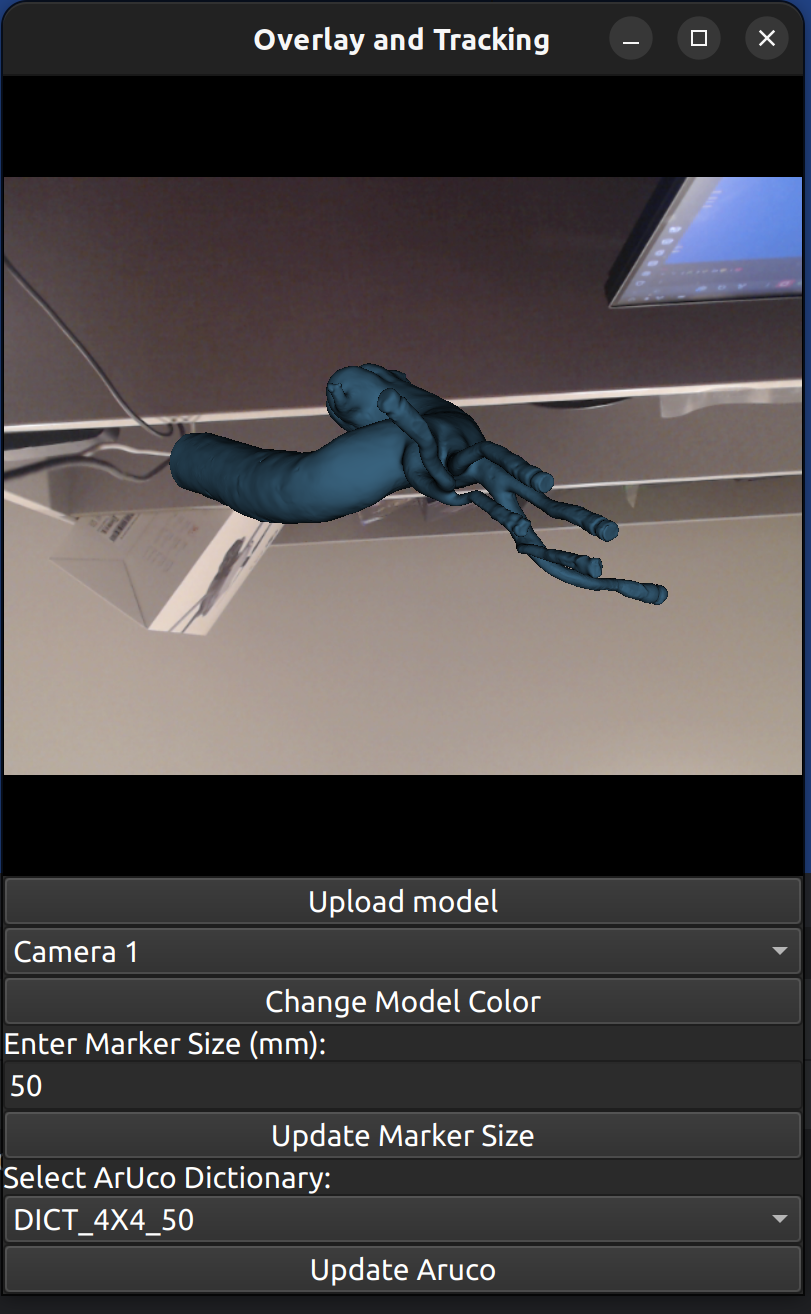
\includegraphics[width=0.4\textwidth]{overlay.png}
                              \caption{Overlay and Tracking Main Menu(With Overlay Activated)}
                        \end{figure}
                        % 模型颜色修改截图展示
                        \begin{figure}[H]
                              \centering
                              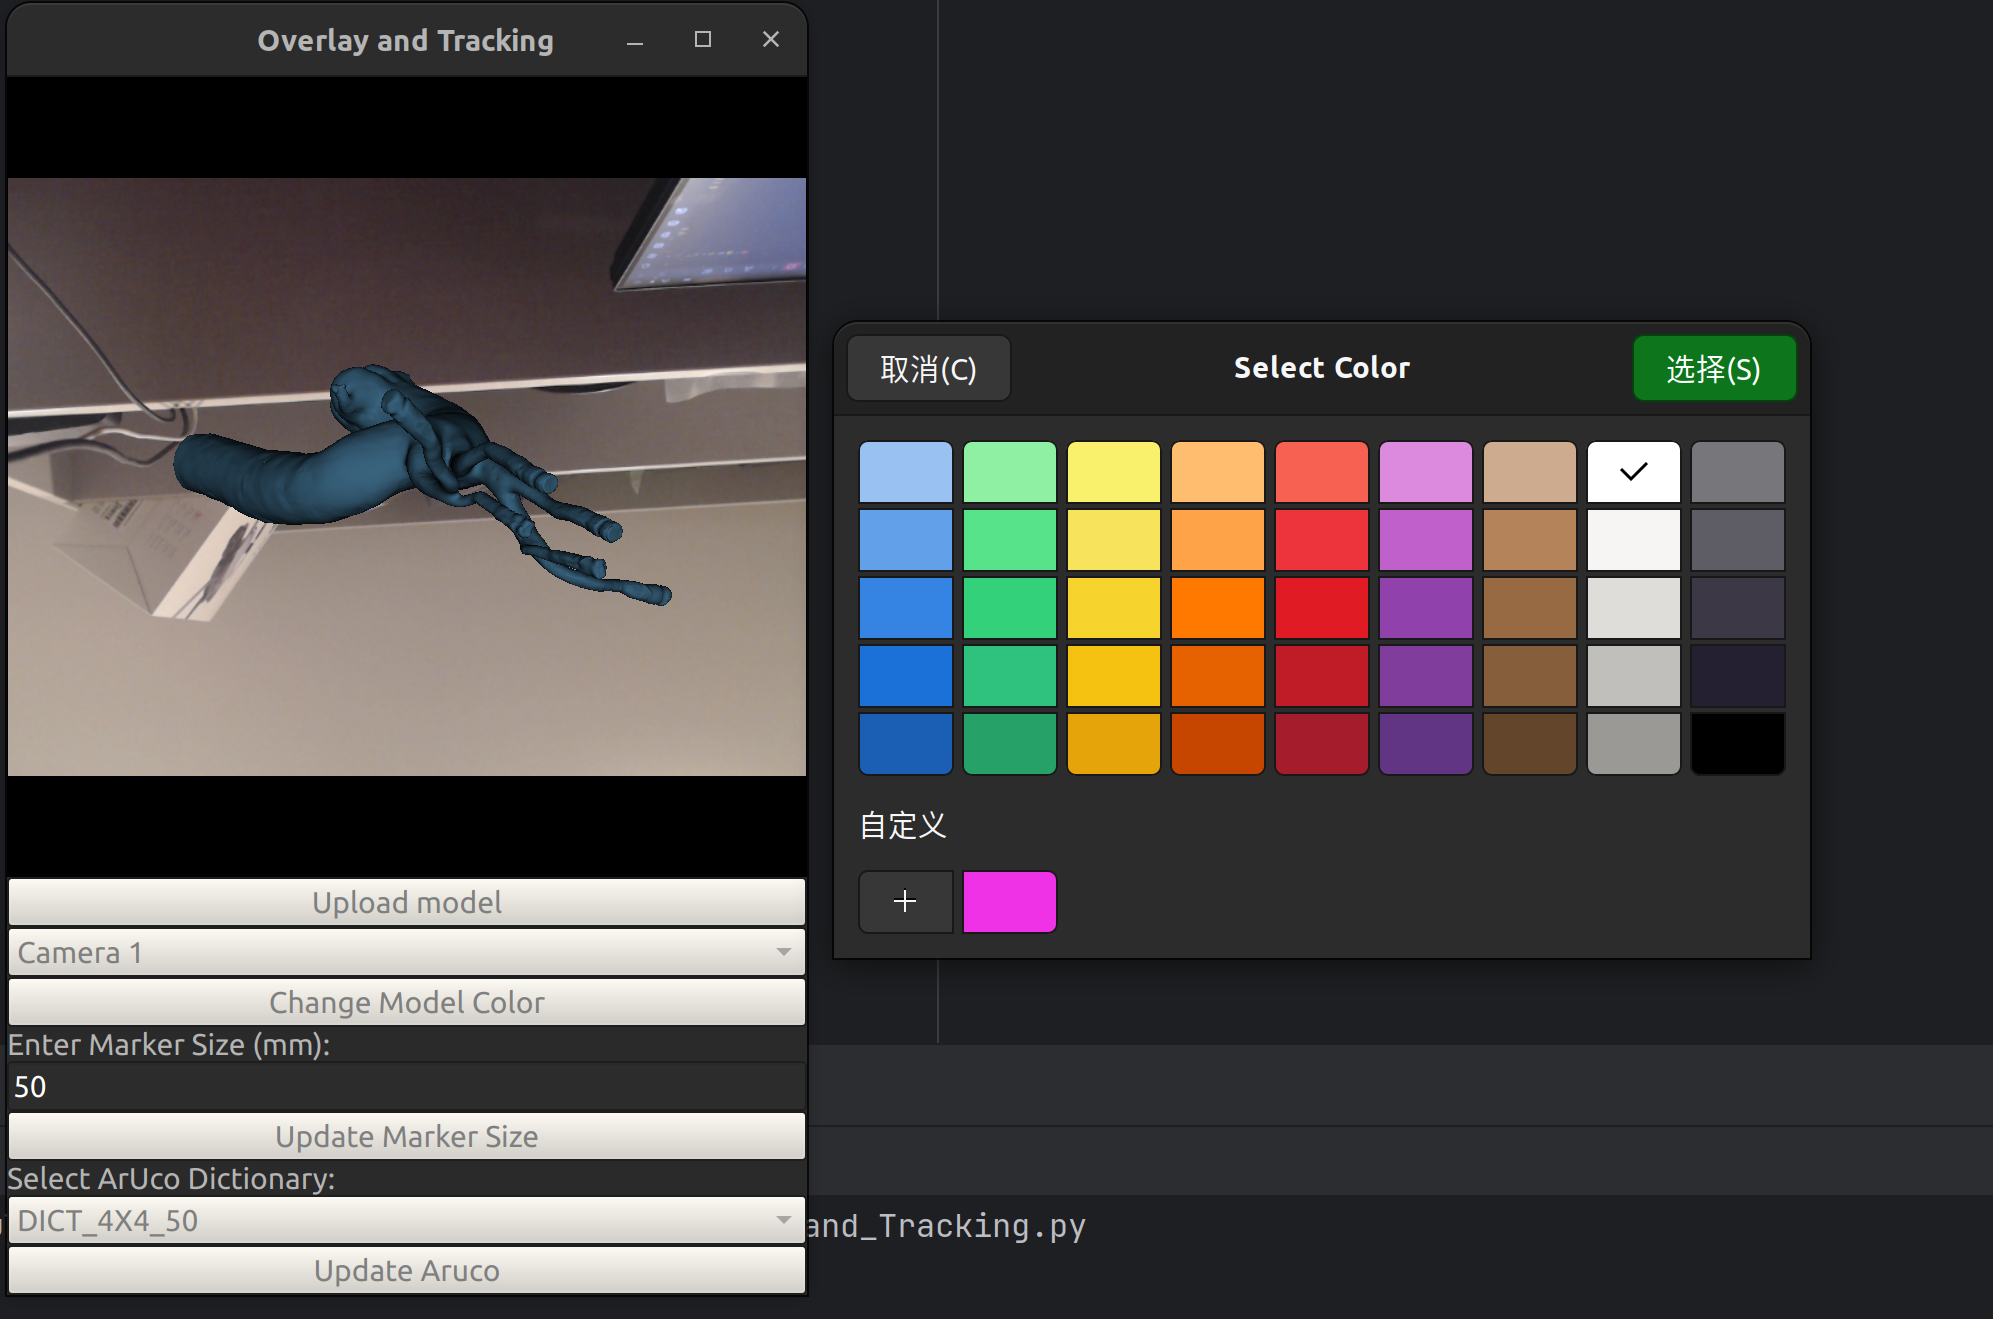
\includegraphics[width=0.6\textwidth]{coulor.png}
                              \caption{Model Color Change}
                        \end{figure}
                        % 视频源切换截图展示
                        \begin{figure}[H]
                              \centering
                              \includegraphics[width=0.4\textwidth]{stream_change.jpg}
                              \caption{Video Source Switching}
                        \end{figure}
                        % 视频上传按钮截图展示
                        \begin{figure}[H]
                              \centering
                              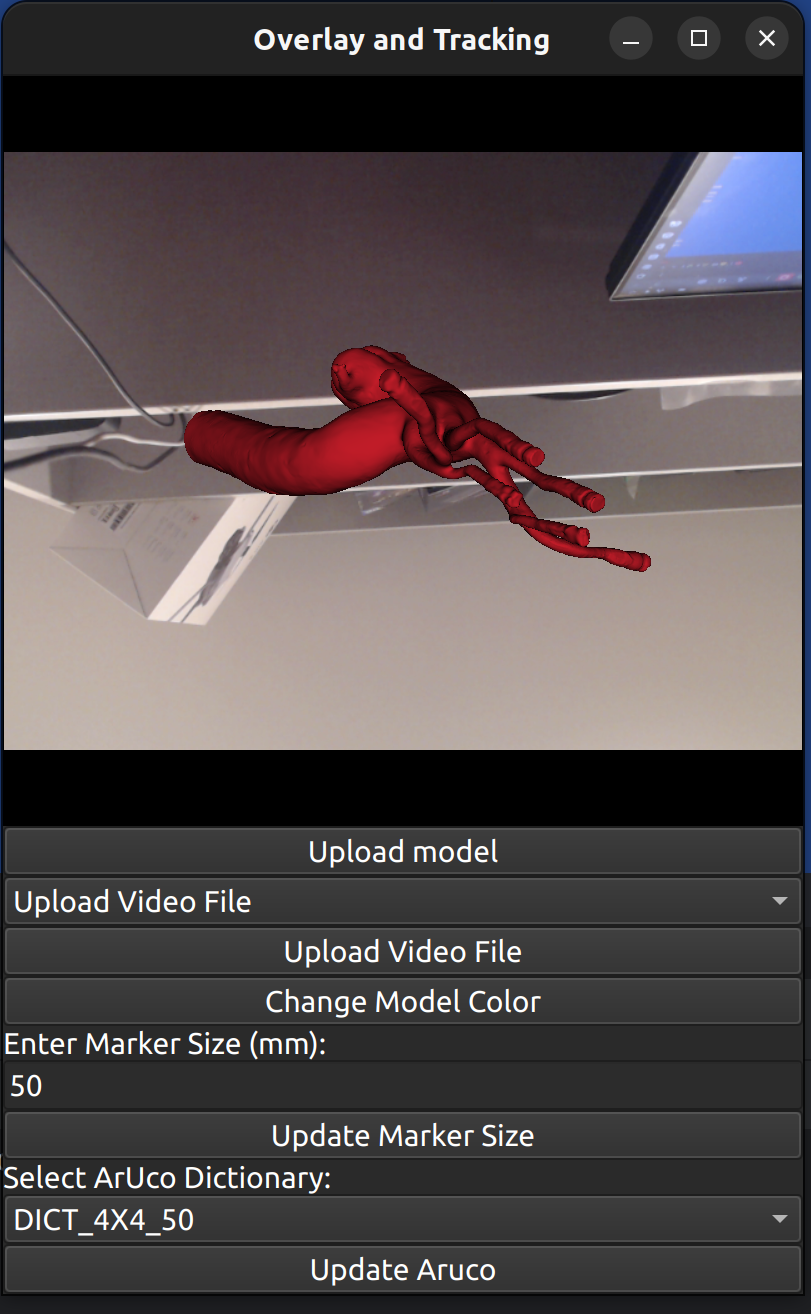
\includegraphics[width=0.3\textwidth]{upload.png}
                              \caption{Color Changed and Video Upload Button}
                        \end{figure}
                        % 选择ArUco字典截图展示
                        \begin{figure}[H]
                              \centering
                              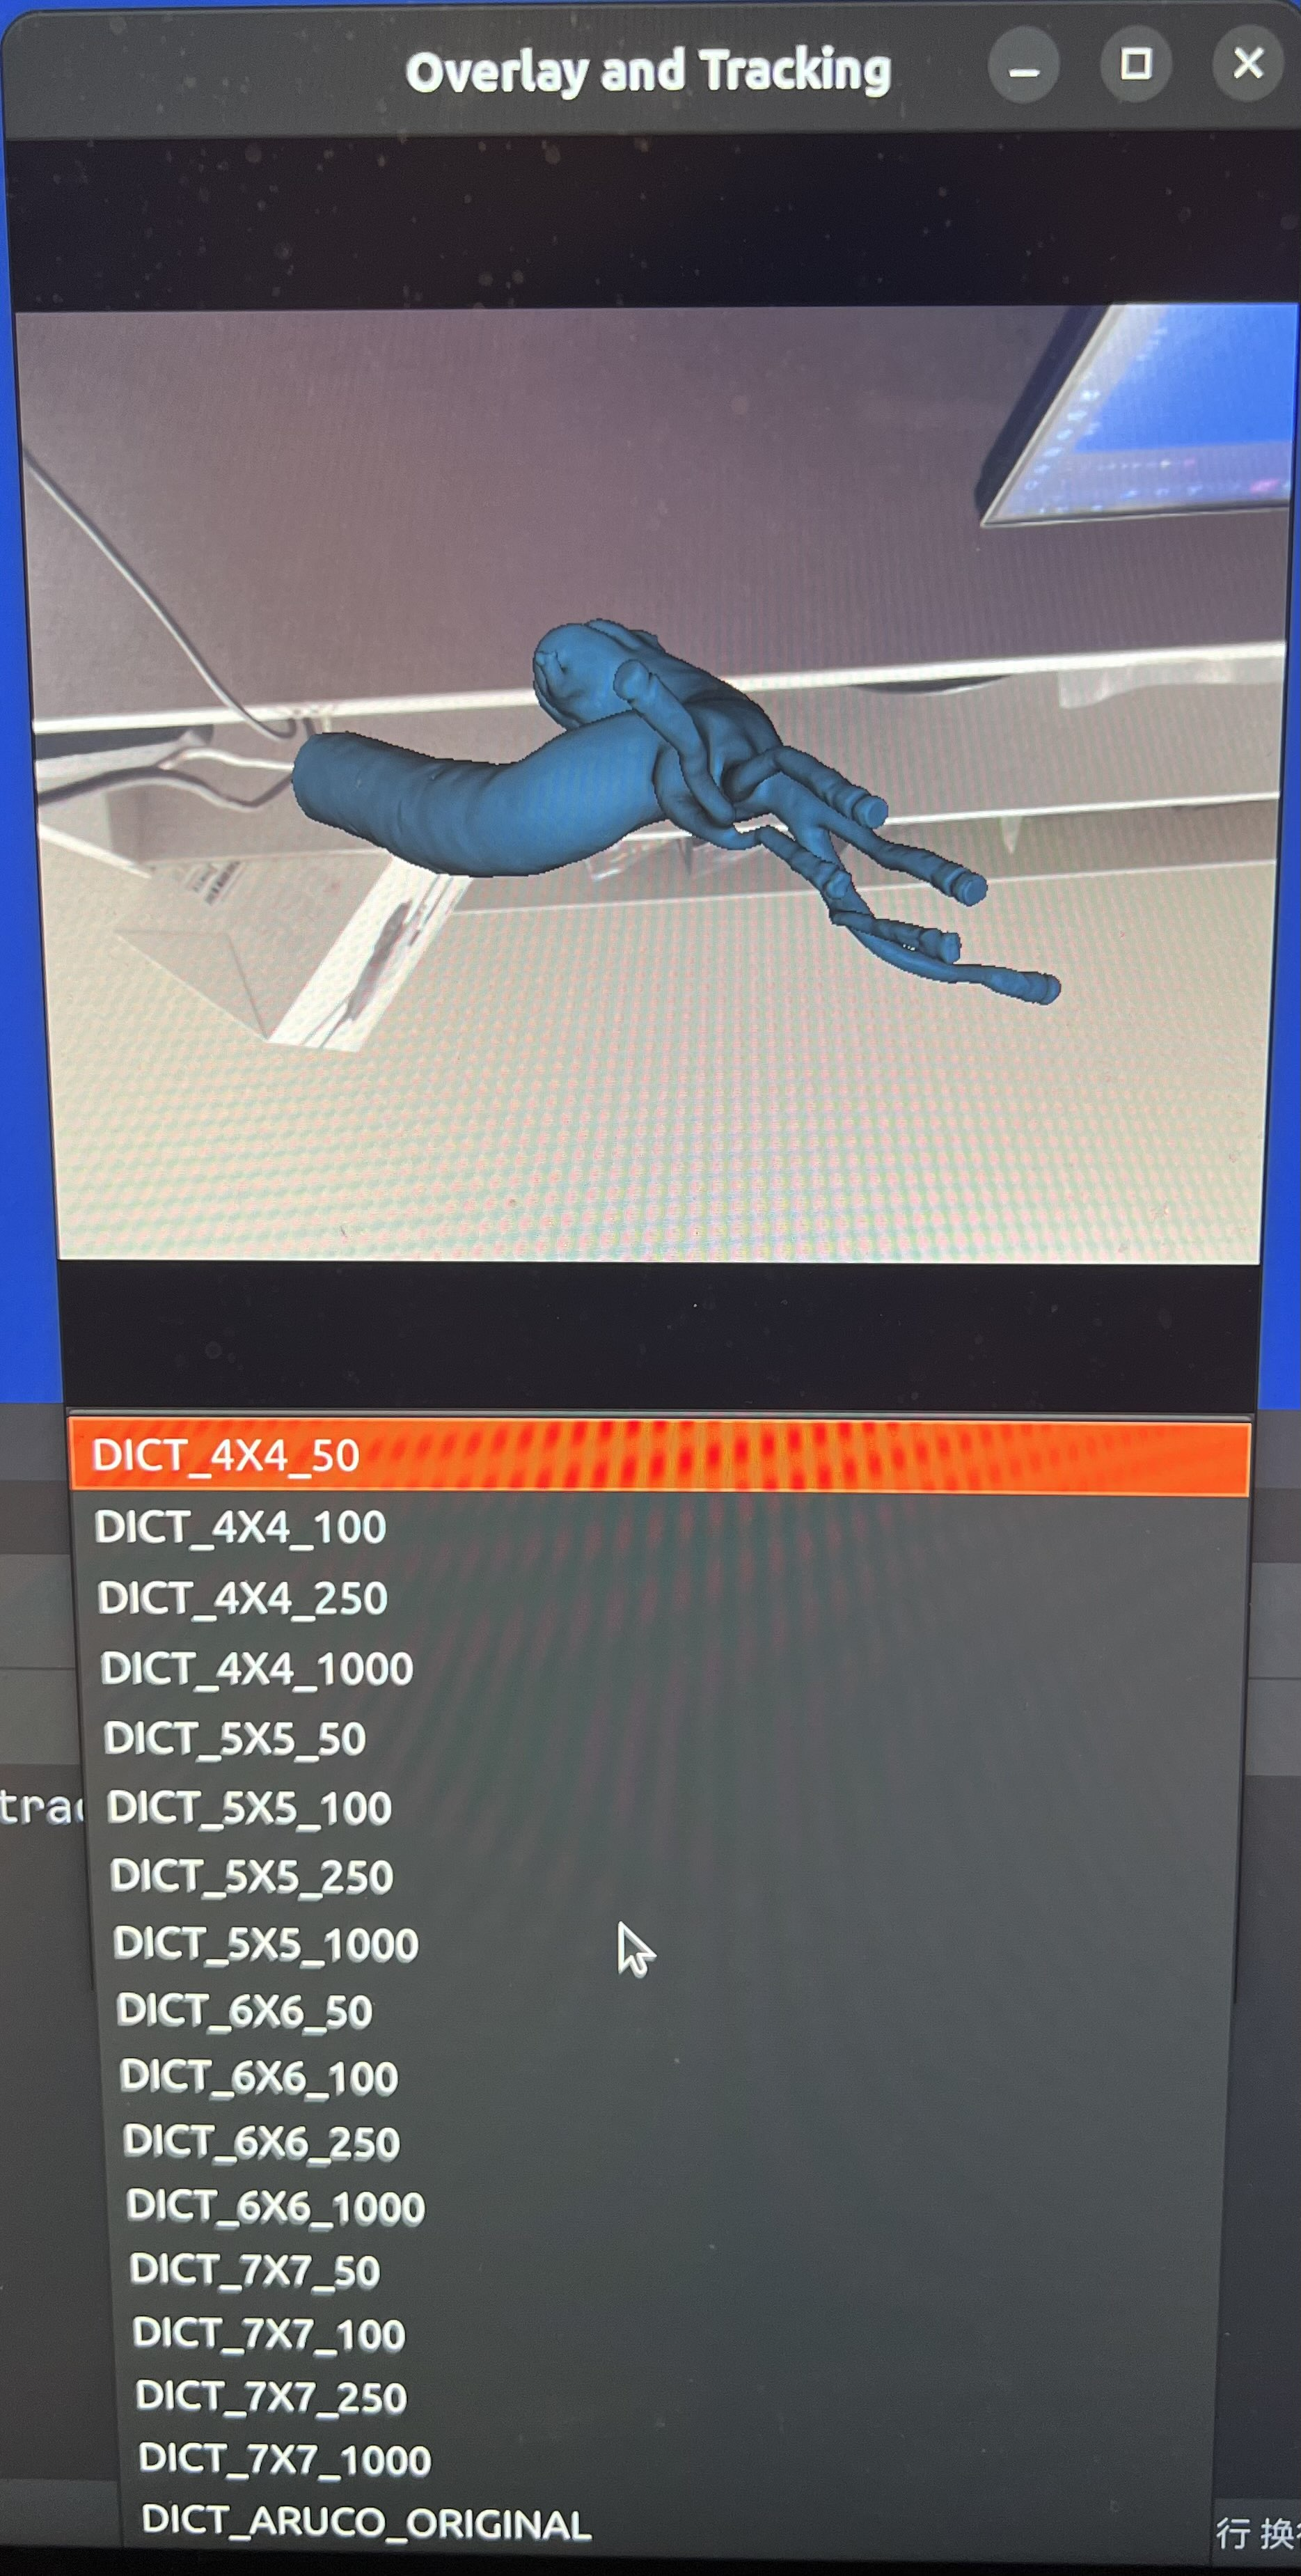
\includegraphics[width=0.3\textwidth]{select_aruco.jpg}
                              \caption{ArUco Dictionary Selection}
                        \end{figure}
                        % 视频上传后展示
                        \begin{figure}[H]
                              \centering
                              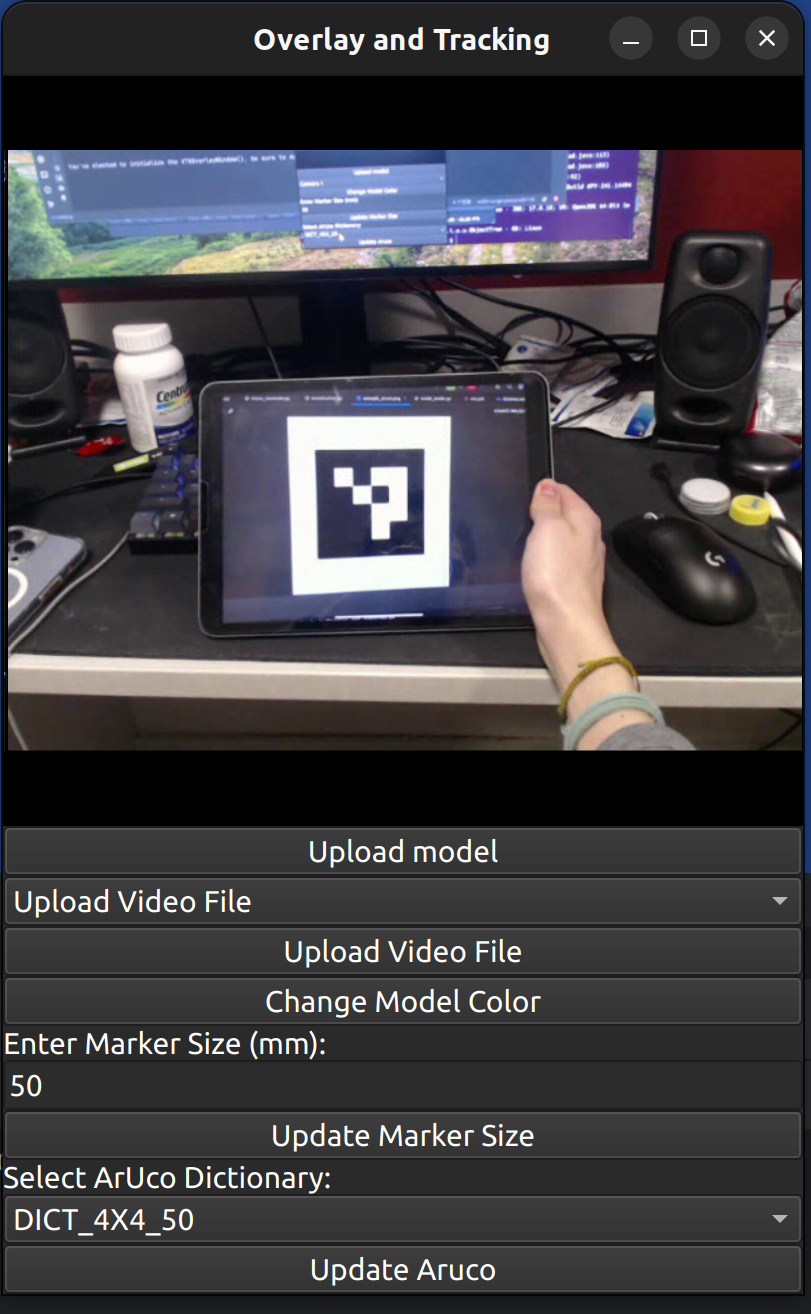
\includegraphics[width=0.4\textwidth]{vedio.png}
                              \caption{Video Upload}
                        \end{figure}
                        % Aruco 修改后展示
                        \begin{figure}[H]
                              \centering
                              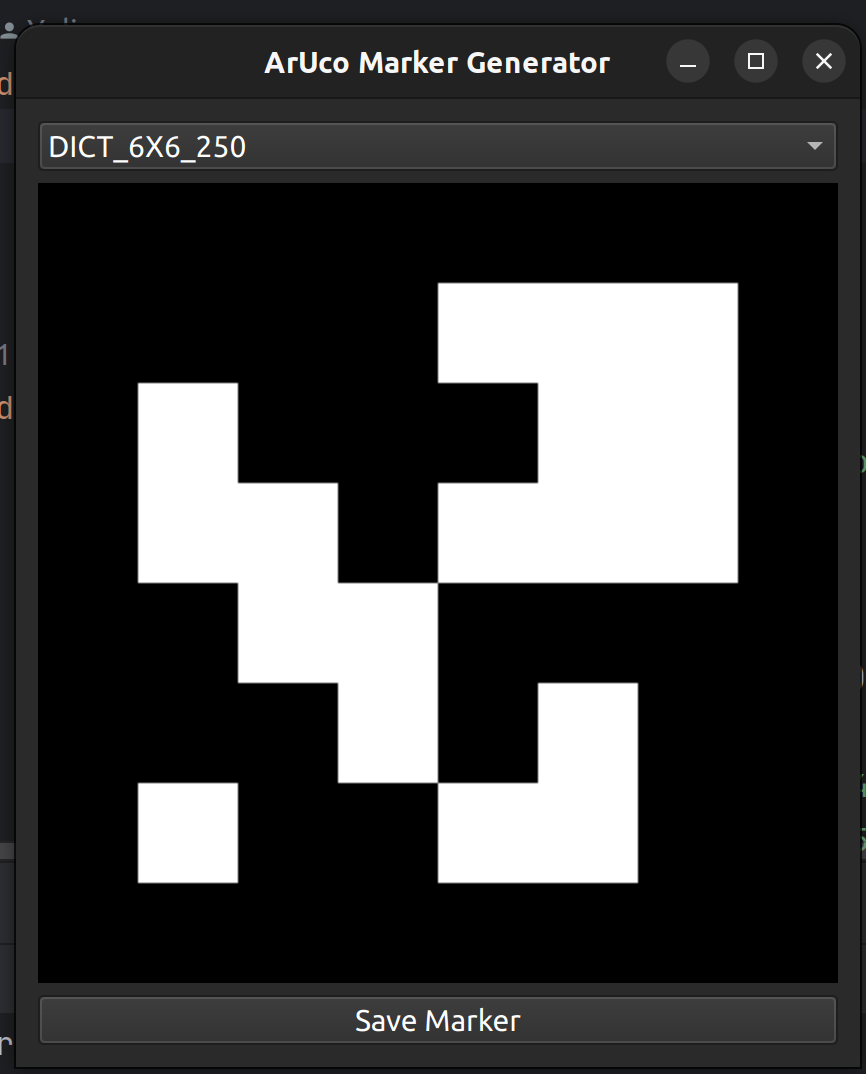
\includegraphics[width=0.4\textwidth]{change_aruco.png}
                              \caption{ArUco Dictionary Changed}
                        \end{figure}
                        % ArUco 保存
                        \begin{figure}[H]
                              \centering
                              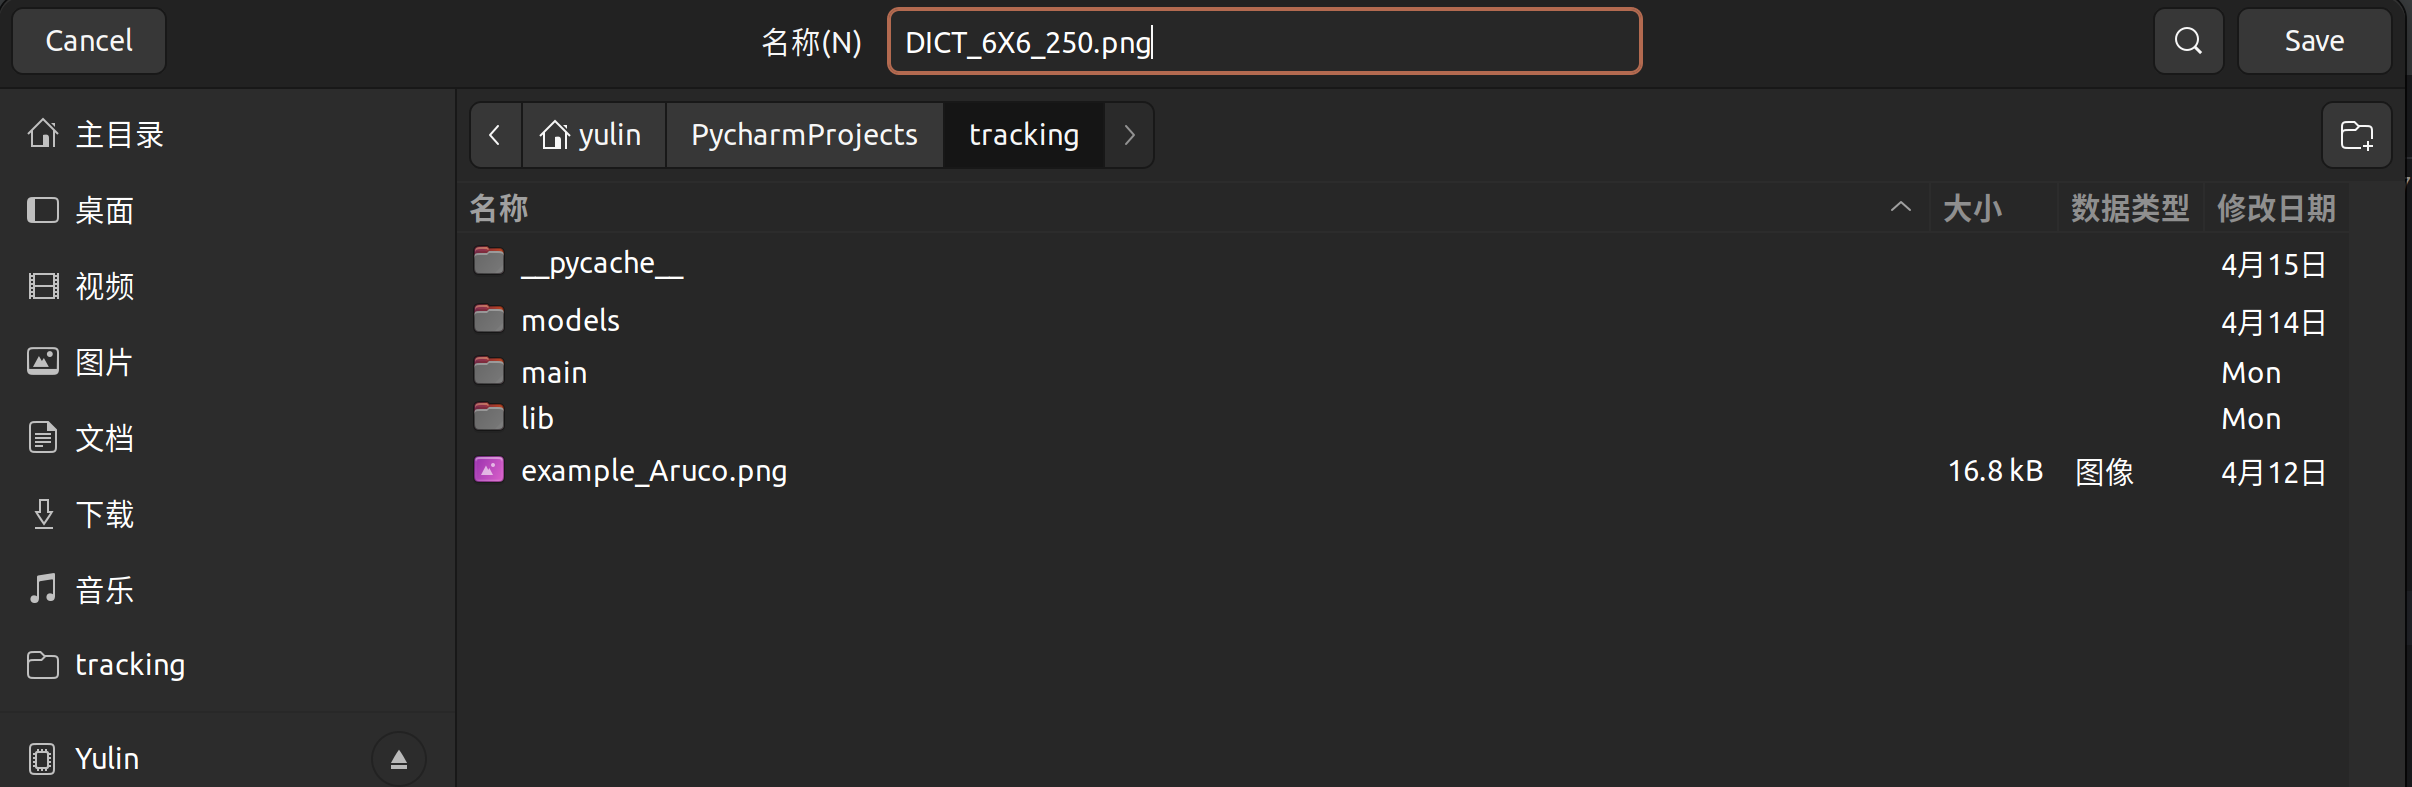
\includegraphics[width=1.2\textwidth]{save.png}
                              \caption{ArUco Marker Saved}
                        \end{figure}
            \end{enumerate}


      \item \textbf{Design Notation and Diagrams}
            \begin{enumerate}
                  \item \textbf{Use Case Diagrams}
                        \begin{figure}[H]
                              \centering
                              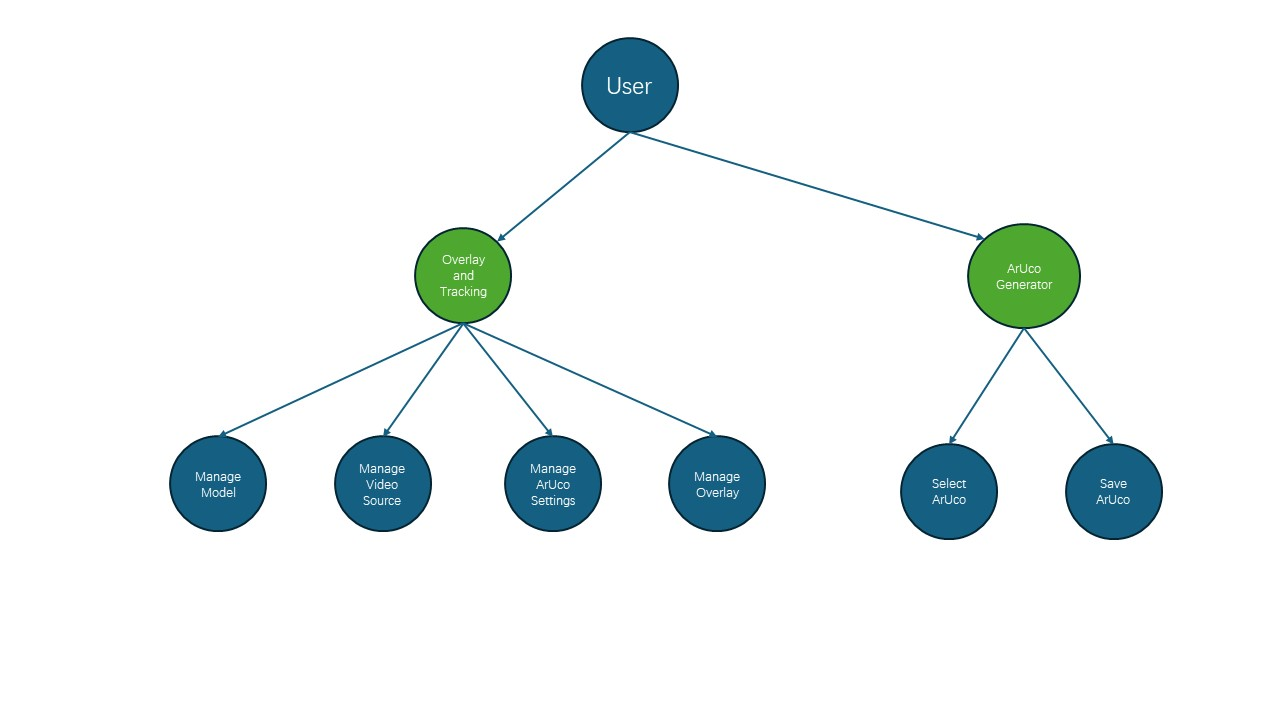
\includegraphics[width=1.1\textwidth]{case.jpg}
                              \caption{Use Case Diagrams}
                        \end{figure}
                  \item \textbf{Data Flow Diagrams}
                        % 提供系统关键部分的伪代码及数据流图。
                        \begin{figure}[H]
                              \centering
                              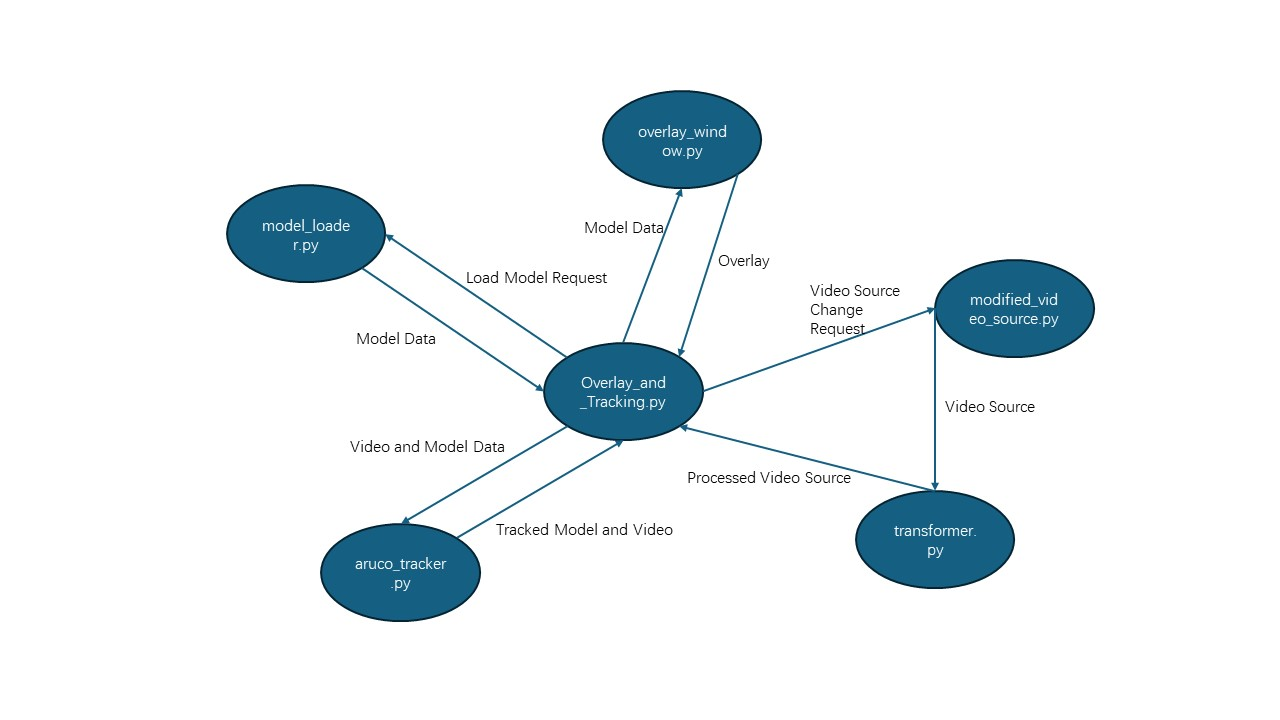
\includegraphics[width=1.1\textwidth]{data.jpg}
                              \caption{Data Flow Diagrams}
                        \end{figure}
            \end{enumerate}
\end{enumerate}

\subsubsection{Implementation}
\begin{enumerate}

      \item \textbf{Backend Implementation}
            % 详细说明系统所使用的数据结构和算法。
            \begin{enumerate}
                  \item \textbf{Pre-processing for video capture and upload}
                        \\\\
                        This part is mainly controlled by \emph{video\_source.py} and is combined with a front-end Qt-based user interface to manage the core video processing functions. A robust video source management and processing system is implemented in \emph{video\_source.py} through the \emph{TimestampedVideoSource} class and \emph{VideoSourceWrapper} class. The system allows the user to interactively control the selection of video sources through a graphical interface, and it ensures accurate video stream processing.
                        \begin{itemize}
                              \item \textit{Video Source Configuration and Management:}
                                    \\
                                    The \emph{TimestampedVideoSource} class uses the OpenCV library's, emph{cv2.VideoCapture} method to initialise the video capture from the camera number or file path. It can support basic video capture functionality or provide the ability to validate the size of the video stream to ensure that the resolution is compatible with the system. If the resolution size provided by the setting is valid, the system sets the resolution accordingly. If the resolution is not valid, the system uses the camera's settings by default. If the requested resolution option is not supported by the camera, the system throws an error, which effectively prevents runtime problems that may result from unsupported video configurations and increases system stability and reliability.
                              \item \textit{Synchronisation and Timestamping:}
                                    \\
                                     The \emph{TimestampedVideoSource} class also serves to synchronise the video stream with the modelled overlay, embedding a timestamp with the current date and time at each frame captured. Each time a video frame is successfully read, the \emph{datetime.datetime.now()} method gets the current system time. This timestamp is then converted to a string or other format and stored or passed along with the video frame, ensuring that each frame has an exact timestamp. In Augmented Reality (AR) or Virtual Reality (VR) systems, quasi-timestamping this timestamp ensures alignment between the 3D model and the actual environment.With such a timestamping feature, \emph{TimestampedVideoSource} can ensure the synchronisation of the video frames for the subsequent synchronisation of the model overlay.
                              \item \textit{Handles multiple video sources:}
                              \\
                              The \emph{VideoSourceWrapper} class manages multiple video sources, allowing the addition of camera inputs or the uploading of video files, and verifying their existence and compatibility. A centralised method for releasing all video sources is provided in this class to ensure that resources that are no longer needed are managed and cleaned up in a timely manner. Each video source is encapsulated in an instance of the \emph{TimestampedVideoSource } class, which allows each source to be controlled and processed independently. This feature ensures that the system load is at an appropriate level.
                              \item \textit{Retrieve and display video frames:}
                              \\
                              Retrieval of frames is achieved by system calls to the \emph{read()} method of each video source, which is implemented through OpenCV's \emph{ cv2.VideoCapture.read() }. This method captures a single frame from the video source and checks to see if it was successfully captured. If successfully captured, the frame is tagged using the current timestamp, ensuring that each frame has an accurate time reference. When processing multiple video sources, the system ensures synchronisation between frames. Synchronisation of frames is achieved by using the same frame rate setting for all sources and matching frames from different sources with timestamps. This allows for smoothness and synchronisation in the case of multiple video source inputs.
                        \end{itemize}

                        \paragraph{pseudocode for the \emph{video\_source.py}:}
                        \begin{minted}[frame=single, linenos=true, fontsize=\footnotesize]{python}
Class TimestampedVideoSource:
    Initialize(source_num_or_file, optional dims):
        Try:
            Open video source with cv2.VideoCapture(source_num_or_file)
        If source not opened:
            Raise RuntimeError("Failed to open Video camera")

        If dimensions provided:
            Validate and set video resolution:
                Check if dimensions are integers and >= 1
                Set resolution using cv2.VideoCapture properties
                If resolution setting fails:
                    Raise ValueError("Requested resolution not supported")

        Initialize empty frame array based on video dimensions
        Initialize timestamp

    Read():
        Capture frame and current time using cv2.VideoCapture.read()
        If frame captured successfully:
            Update timestamp with current datetime
        Return frame, timestamp

    Release():
        Release video source using cv2.VideoCapture.release()

    Update source(new_source):
        Release current source
        Reinitialize with new source

Class VideoSourceWrapper:
    Initialize():
        Create an empty list for storing video sources

    Add camera(camera_number, optional dims):
        Validate camera input (check if camera number is valid)
        Add camera source with optional dimensions to the list

    Add file(filename, optional dims):
        Validate if filename exists and is a valid file
        Add file source with optional dimensions to the list

    Get next frames():
        For each source in the list:
            If source is opened:
                Read frame from source
            Collect and return all frames

    Release all sources():
        For each source in the list:
            Release source
                        \end{minted}
                  \item \textbf{Image Processing Algorithms in Multi-Layer Video Rendering}
                        % 描述如何存储和处理连续的图像帧,例如使用循环缓冲区或队列来管理实时视频帧。
                        \\ In a video rendering system, video frames need to be dynamically managed to create complex visual effects, such as models and real-time video overlays in this project. This also involved real-time adjustments to the \gls{alpha}\cite{Alpha} and video. A greyscale image with alpha blending of the RGBA stream was used to precisely control transparency and layering effects to enable the superimposition of a layer's frame (e.g. the model) onto the original frame\cite{9979846}. Ensuring overlay accuracy and visual fidelity is crucial for applications such as augmented reality\cite{SETTIMI2022104272}.
                        \\\\
                        In addition, it is necessary to update and align the video frames to the appropriate layers by adjusting the data range according to the size of the incoming video frames. This incorporation of real-time processing improves the continuity of the video image by preventing visual interruptions caused by frame misalignment\cite{Wang}.
                        \\\\
                        I also introduced \gls{aesl} into the multi-layer video rendering system (\emph{Overlay\_and\_Tracking.py}). This enhances image processing, such as when processing video streams involving complex dynamic scenes\cite{7410724}. By dynamically adjusting its smoothing parameter (Alpha), \gls{aes} is able to more accurately adapt to changes in content within a video frame, such as lighting adjustments, scene switching, or object movement, and can reduce visual jitter and blurring due to rapid changes \cite{7410724}.
                        \\\\
                        Compared with the traditional \gls{emal}, the adaptive feature of AES has a greater advantage. \gls{ema}, although fast in processing and low in computational cost, may not be able to adequately adapt its fixed smoothing parameters to real-time changes in the video content in the face of complex scene variations, thus affecting the final image quality\cite{aes,aes2,InvestopediaEMA}.
                        In a multilayer rendering system, combining AES for real-time video transmission and dynamically adjusting the smoothing parameters according to the content differences between the previous and previous frames can maintain the continuity and naturalness of the visual effects, especially when dealing with moving objects and changing backgrounds. In addition, AES's also better handles scenes with large lighting variations, maintaining the balance of colors and shades of light and dark \cite{7298776}.
                        \\\\
                        I have similarly experimented with \gls{cesl}, and while it excels in handling data with clear trends and cyclical variations, its application in video rendering systems may not be as straightforward and effective as AES. Because \gls{ces} is designed to provide a more comprehensive understanding of the multiple influences on the data \cite{ComplexES2018,Complex}, its use in non-predictive applications may lead to overly complex processing and increased computational burden.
                        \\\\
                        Therefore, AES is ultimately used in video rendering systems to respond more directly to real-time changes in video content, reduce visual jitter, and improve the viewing experience.
                        \\\\
                        To summarize, AES can improve image stability and visual quality, as well as enhance the system's responsiveness to environmental changes. By intelligently adjusting processing parameters, AES helps to ensure high efficiency while also adapting to visual jitter or lighting changes that may be encountered with ArUco marker tracking.
                        \paragraph{Code for the AES:}
                        \begin{minted}[frame=single, linenos=true, fontsize=\footnotesize]{python}
class SmoothedTransform:
    def __init__(self, alpha, min_alpha=0.01, max_alpha=0.9):
        """
        Initializes the adaptive smoothing transform class.
        
        Parameters:
        alpha (float): The initial smoothing factor.
        min_alpha (float): The minimum allowable value for alpha 
        to prevent it from becoming too low.
        max_alpha (float): The maximum allowable value for alpha 
        to prevent it from becoming too high.
        """
        self.alpha = alpha
        self.min_alpha = min_alpha
        self.max_alpha = max_alpha
        self.transform = None
      def adjust_alpha(self, new_transform):
            """
            Adjusts the smoothing factor alpha based on the 
            difference between the new transform and the 
            current transform to 
            better adapt to recent data changes.
                                          
            Parameters:
            new_transform (float): The new data point used to 
            update the transform.
            """
            if self.transform is not None:
            # Calculate the absolute difference between the current 
            # and new transforms
            error = abs(new_transform - self.transform)
            # Dynamically adjust alpha based on the error, 
            # inversely scaling it
            self.alpha = max(self.min_alpha, min(self.max_alpha, 
            1 / (1 + error)))
                              
      def update(self, new_transform):
            """
            Updates the current transform with a new data point using
            adaptive exponential smoothing.
                                          
            Parameters:
            new_transform (float): The new data point to incorporate
            into the smoothed data.
                                          
            Returns:
            float: The updated transform value.
            """
            if self.transform is None:
            # If no transform has been set yet, initialize it 
            # with the new transform
            self.transform = new_transform
            else:
            # Adjust alpha based on the new data point
            self.adjust_alpha(new_transform)
            # Apply the adjusted alpha to compute 
            # the new smoothed transform
            self.transform = self.alpha * new_transform + 
            (1 - self.alpha) * self.transform
            return self.transform
                              \end{minted}
                  \item \textbf{Model Rendering and Overlay}
                        % 详述用于检测和追踪ArUco标记的算法,包括图像分割、模式识别和机器学习技术。
                        
                        \begin{itemize}
                              \item 
                        \end{itemize}
                  \item \textbf{Marker Detection and Tracking}
                        % 介绍如何将三维模型精确地放置在虚拟环境中,可能涉及计算几何和物体识别算法。

                  \item \textbf{Model Color change}
                        % 分析关键算法的时间和空间复杂度,讨论在不同操作环境(如不同硬件或软件平台)下的性能表现。
                  \item \textbf{ArUco Marker Settings}
                        % 详细说明系统的用户界面设计和实现

                  \item \textbf{ArUco Generator}

            \end{enumerate}
      \item \textbf{Frontend Implementation}
            % 详细说明系统的用户界面设计和实现。
            %通过用户界面进行交互式控制:
            %在用户界面中,用户可以通过一个下拉菜单(QComboBox)从可用视频源中进行选择,并且对于基于文件的视频源,一个上传按钮(QPushButton)允许用户通过文件对话框选择并上传视频文件。视频源选择的变更会触发后端VideoSourceWrapper类的更新,该类管理多个视频源,提供灵活性并增强用户交互。这种设计使用户可以轻松切换视频输入源,并根据需要上传自定义内容。
\end{enumerate}

\subsection{Part2: Endovascular Intervention Simulation}
% 在这里详细介绍关于“Endovascular Intervention Simulation”的设计和实现。

\subsubsection{Design}
% 描述“Endovascular Intervention Simulation”部分的设计细节。

\subsubsection{Implementation}
% 描述“Endovascular Intervention Simulation”部分的具体实现细节。


% Testing & Evaluation
\section{Testing \& Evaluation}

% Project Ethics
\section{Project Ethics}
I have read and abide by the University’s ethical guidelines\cite{UoL_COMP390_2023-24}. The project did not involve direct interaction with human
participants during the design, implementation or evaluation phases. An extensive review of the project scope and methodology
confirmed that no personal data was collected, analyzed or used. In addition, all activities were within the scope of activities
permitted by our ethical guidelines. It was verified with the project supervisor that no customized activities required separate
ethical approval. Therefore, there are no other ethical issues involved in this project.
% Conclusion & Future Work
\section{Conclusion \& Future Work}
\subsection{Conclusion}

\subsection{Future Work}

\section{BCS Criteria \& Self-Reflection}
This section will be used to state that my project met the six outcomes expected by the Chartered Institute of Information Technology\cite{BCS2020}.
I will focus on illustrating an ability to self-manage a significant piece of work and the critical self-evaluation component.
\subsection{An Ability to Apply Practical and Analytical Skills during the degree programme.}
The project has demonstrated the practical and analytical skills I have learnt during my time at university. Throughout the degree I have gained a deeper understanding of programming languages such as Python, C\# , Java and C\+\+ and have gradually begun to experiment with them. The theoretical and practical foundations of these languages have been key in enabling me to achieve the complex functionality required for development and realisation projects. For example, in the Part1: Real-world Model Interaction and Tracking section of my project, which was written entirely in Python, there was a high level of theoretical and practical demand for the Python language. In my Part2: Endovascular Intervention Simulation, I needed to acquire and apply knowledge such as the application of Unity and the development and application of the C\# language that I had learnt in my degree programme. These technical skills were acquired and refined through a careful learning process and were directly applied to the project, which dealt with the development of a real model interaction and tracking system and the development of a Unity-based Endovascular Intervention Simulation.
\\\\
In developing Part1: Real-world Model Interaction and Tracking and Part2: Endovascular Intervention Simulation, I have also made extensive use of the Artificial Intelligence, Game Development and Computer Vision knowledge that I have learnt on my degree course.
\\\\
For Part1: Real-world Model Interaction and Tracking, I utilised the techniques learnt in the Computer Vision course to process the images and used the OpenCV package usage learnt in the course to implement the tracking of the ArUco markers. By utilising the image processing and tracking capabilities of OpenCV, accurate model interaction in complex environments is carried out in practice.
\\\\
In Part2: Endovascular Intervention Simulation, I used my knowledge of game development to develop a Unity project, using \gls{blender} to modify and optimise the model, and applying Unity techniques to ensure that Rope interacts with the blood vessels.
\\\\
This project, dedicated to the development of a realistic simulation used for endovascular interventions in a virtual reality environment, emphasised my ability to integrate practical skills and theoretical insights, demonstrating a deep understanding of the technical and theoretical aspects I have learnt during the course.
\\\\
Overall, this project clearly demonstrated my ability to apply the analytical and practical skills acquired during my degree programme. It also demonstrated my understanding and use of complex programming techniques and frameworks, as well as my ability to use multidisciplinary knowledge to cross-cut problem solving. Through this project, I have accomplished the ability to translate my learning into practical applications in the real world.



\subsection{Innovation and/or Creativity}
There are some innovations in the field of medical simulation technology in my project, especially Part2: Endovascular Intervention Simulation, The aim of Part2 is to create one of the few open source endovascular intervention simulation projects in the field to make training tools more accessible to the medical community. The project combines traditional surgical simulation with augmented reality/virtual reality technology to make surgical simulation procedures visual and easy to practice. Compared to traditional simulations that are limited to 2D screen displays, this approach uses virtual reality to present surgical simulations in 3D space, which not only enhances the realism of the simulation and interactions, but also allows users to experience and understand the steps involved in the surgery more clearly by allowing them to interact with the simulated environment in a more intuitive and natural way.
\\\\
The project uses an open source framework (\gls{mrtk}) and the integration of Augmented Reality/Virtual Reality (AR/VR) technology to provide a practical and innovative application for educational tools in the medical field.


\subsection{Synthesis of Information, Ideas, and Practices}
This project integrates development tools and theoretical principles from different fields to design the open source Endovascular Intervention Simulation to provide a convenient tool for medical surgery simulation or surgical training.
\\\\
In the first part of the project, Real-world Model Interaction and Tracking, open source development tools such as OpenCV, VTK and SciKit-Surgery were used. The use of these powerful tools allows me to design user-friendly graphical interfaces or to enhance the model rendering capabilities and real-world model tracking capabilities of my application. OpenCV provides a rich set of image processing tools to help me perform complex image processing and tracking, while VTK and SciKit-Surgery provide powerful tools for medical impacts, such as multilayer image rendering and overlays. This can help me combine tracking capabilities with augmented reality to create a more interactive virtual reality system for users. This section combines knowledge, tools and ideas from various fields to create a high quality solution.
\\\\
Part 2: Endovascular Intervention Simulation Developing an application on \gls{holo} using \gls{mrtk} translates the theoretical knowledge I have learnt in my school course such as C\# and Unity development into a practical solution. The development utilised model modification and knowledge related to Unity development, C\# development, etc. to transform Endovascular Intervention Simulation, which is traditionally limited to a flat display, into a virtual reality simulation with immersive, interactive features. This part of the development demonstrates how AR application development techniques and Unity development can be combined to provide a virtual reality surgical simulation with multiple functionalities.
\\\\
Both parts of the project exemplify how technical and theoretical knowledge from the fields of computer vision, artificial intelligence and software development can be applied to create effective and innovative medical training tools.
\subsection{Meeting a Real Need in a Wider Context}
Both parts of the project, Part1: Real-world Model Interaction and Tracking and Part2: Endovascular Intervention Simulation, address some of the broader needs in the medical field.
\\\\
For Part1: Real-world Model Interaction and Trac, current market systems usually lack user-friendly graphical interfaces, and features such as model colour, selection of different ArUco markers, and resizing are lacking or incomplete, which can cause some degree of difficulty for users. For Part1 the project adds a graphical interface and provides a variety of modifiable parameters to optimise these shortcomings, making the software less difficult to use and better adapted to the needs of a wide range of scenarios.
\\\\
Part2 considers the lack of open source endovascular intervention simulation in the market and the fact that most existing simulation tools are limited to 2D planar presentation and cannot meet the complex 3D visual and operational needs. The aim is to develop an open source platform that supports immersive 3D simulation, AR/VR and other functions. The system can support 3D simulation in AR/VR (deployed in Microsoft \gls{holo}), and by lowering the barrier to use through more intuitive and simple controls, it can be used in the future to allow healthcare professionals or non-professionals alike to experience or learn surgical skills. This simulation tool can not only be used for professional training, but also meets the need for telemedicine services that can provide remote diagnosis and treatment in the future.
\\\\
Overall, it is planned that these two components will be combined in future work, which can meet the needs for simulation of surgical training simulation for simplicity, remote operation, and 3D highly experiential simulation. In the future it may be possible to expand into more areas to meet a wider range of needs, such as providing an immersive experience of Endovascular Intervention Simulation for lay people.

\subsection{An Ability to Self-Manage a Significant Piece of Work}
In my project I demonstrated the ability to self-manage a significant piece of work, but it was partially flawed. The project consisted of two widely differing parts, which added to the difficulty of managing the project as a whole, and in order to keep both of the major parts of the project accurately planned and executed, I used a variety of tools and methods to ensure that the project ran smoothly.
\\\\
Firstly, I used a number of time management tools to map out the timeline of the project, including key milestones, time required, and deadlines for each progress module. I created some Gantt charts and schedules to help me monitor the progress of the project and try my best to make sure that the tasks in each phase are completed on time. In this way I could get a clear picture of the overall progress of the project and adjust the plan as much as possible in time to cope with possible delays. However, as this was my second time working on a larger volume project (the last time was COMP208 Group Project), I was not able to be very perfect in creating the schedule and Gantt chart, and some mistakes were made.
\\\\
Secondly, in terms of project management, I used \gls{git} to maintain version control of the project and writing between team members. I used GitHub to effectively track code updates and backups, as well as to enable team members to view the latest progress of the project in real time and provide feedback. GitHub's version control and backup features have many times saved errors caused by mistakes, effectively avoiding many accidents. Using this open source platform has helped me to manage a major task and increase the efficiency of multi-person collaboration.
\\\\
In addition, in order to control the development progress and quality, I also hold weekly progress meetings with my team members and supervisor to report the progress of this week's work and discuss and plan the next work. In these meetings, I can get sufficient feedback to help me modify and optimise my previous work, and make reasonable planning and arrangement for the next work. This regular reporting and discussion has ensured that the project has developed according to the set objectives.
\\\\
I also focus on stage-by-stage problem analysis and risk management during project implementation. Whenever the project progresses to a certain stage, I will review the previous work, check and improve any possible problems in the completed work, and make sure that the previous work is accurate before proceeding to the next stage1. This is a good way to ensure that I make fewer mistakes when managing a large volume of work.
\\\\
Whilst I have adopted a variety of methods during the project management process to ensure that the project is executed efficiently and to a high quality as planned, I still have some shortcomings in my ability to self-manage a significant piece of work. For example, although I produced a Gantt chart and schedule to monitor the progress of the project, at the beginning of the project I did not properly consider the time required for some parts and the difficulties I may have encountered, for example, I encountered great difficulties in carrying out the initial design and import of the Rope in Part2: Endovascular Intervention Simulation, etc., and the rate of progress was not as fast as expected. This resulted in the project progressing at a much slower pace than expected and led to the project being put on hold for some time. In addition, although we had weekly meetings, some of them were of minimal effect. These meetings usually took place when the project was experiencing some major difficulties, and in these meetings the solutions to the problems and the planning for the next phase of the project progress were not discussed very effectively.
\\\\
In addition, I had problems with teamwork when using GitHub for project management. Poor documentation, different operating systems used by each member, conflicting versions of various software packages, and GitHub's file size limitations for uploading files caused many difficulties for team members when sharing through GitHub.
\\\\
Overall, this project demonstrated my ability to self-manage a significant piece of work, but it also demonstrated my shortcomings in some of these areas. This project gave me a great opportunity to optimise my ability to manage projects, such as time planning skills and communication with team members, as well as making me realise what I need to learn and improve in project management.
\subsection{Critical Self-Evaluation of the Process}
In my projects, Part1: Real-world Model Interaction and Tracking and Part2: Endovascular Intervention Simulation, although both have been accomplished, there have been many challenges and difficulties in the development process, and so far there have been some shortcomings. Through in-depth critical self-evaluation, I was able to comprehensively analyse the successes and shortcomings of the project, as well as gain experience and lessons learned.
\\\\
First of all, the functionality of my project Part1 is relatively complete, which can effectively implement real-time model overlay and ArUco marker tracking, and complete the basic function of my plan. At the same time, I also added extra features such as ArUco icon parameter tuning and ArUco icon generator. However, there are some technical limitations in this part, mainly in platform compatibility. Currently, the system only runs on the Linux platform and has not yet implemented support for other operating systems such as Windows or macOS, nor has it been able to complete deployment on VR/AR devices such as HoloLens. This limitation may have impacted the project's widespread adoption. In this regard, I believe that my Part1 met the requirements of my plan, but still needs to be improved and extended in terms of compatibility.
\\\\
For Part2, the development process encountered significant technical challenges, especially during the stages of designing the Rope and developing the method of interaction between the Rope and the vessel wall. These technical issues led to delays in the development progress and the final product implemented only the most basic functionality and did not achieve the level of Rope-vessel wall interaction required at the beginning of the design. This difficulty stemmed from my lack of skill in using development tools such as Unity and Blender, and my underestimation of the complexity of the interaction logic of physical simulation and model interaction. Nonetheless, the development process has greatly strengthened my technical skills in 3D modelling, Unity development and physics simulation simulation.
\\\\
By critically reflecting on and analysing these issues, I realised that I should plan better in the upfront technical assessment and time management phases when undertaking future project management. This includes analysing in detail the technical difficulty and time required for each development phase during the project planning stage, as well as being prepared in advance to deal with unforeseen circumstances as they occur. In addition, it is also important to communicate more with team members and supervisors at the technical level during the project to accelerate the speed of breaking through the development challenges.
\\\\
Overall, the development process of this project was full of difficulties and challenges, but it also strengthened my technical level, project management skills and the ability to solve unknown problems. Through this project, I was able to improve my professional skills in a variety of different technical areas, as well as develop my ability to effectively self-manage and work in a team on projects with complex environments. Through this critical self-assessment and reflection, I was able to better identify and improve on my shortcomings in my work and prepare myself for the greater challenges I may face in the future.

% References (The bibliography will be printed here)
\printbibliography
\printglossaries

\end{document}
